% ##########################################################################
% ################################### DDL ##################################
% ##########################################################################
\section[DML]{Data-Manipulation-Language}
\label{sec:dml}

\begin{figure}[h]
  \centering
  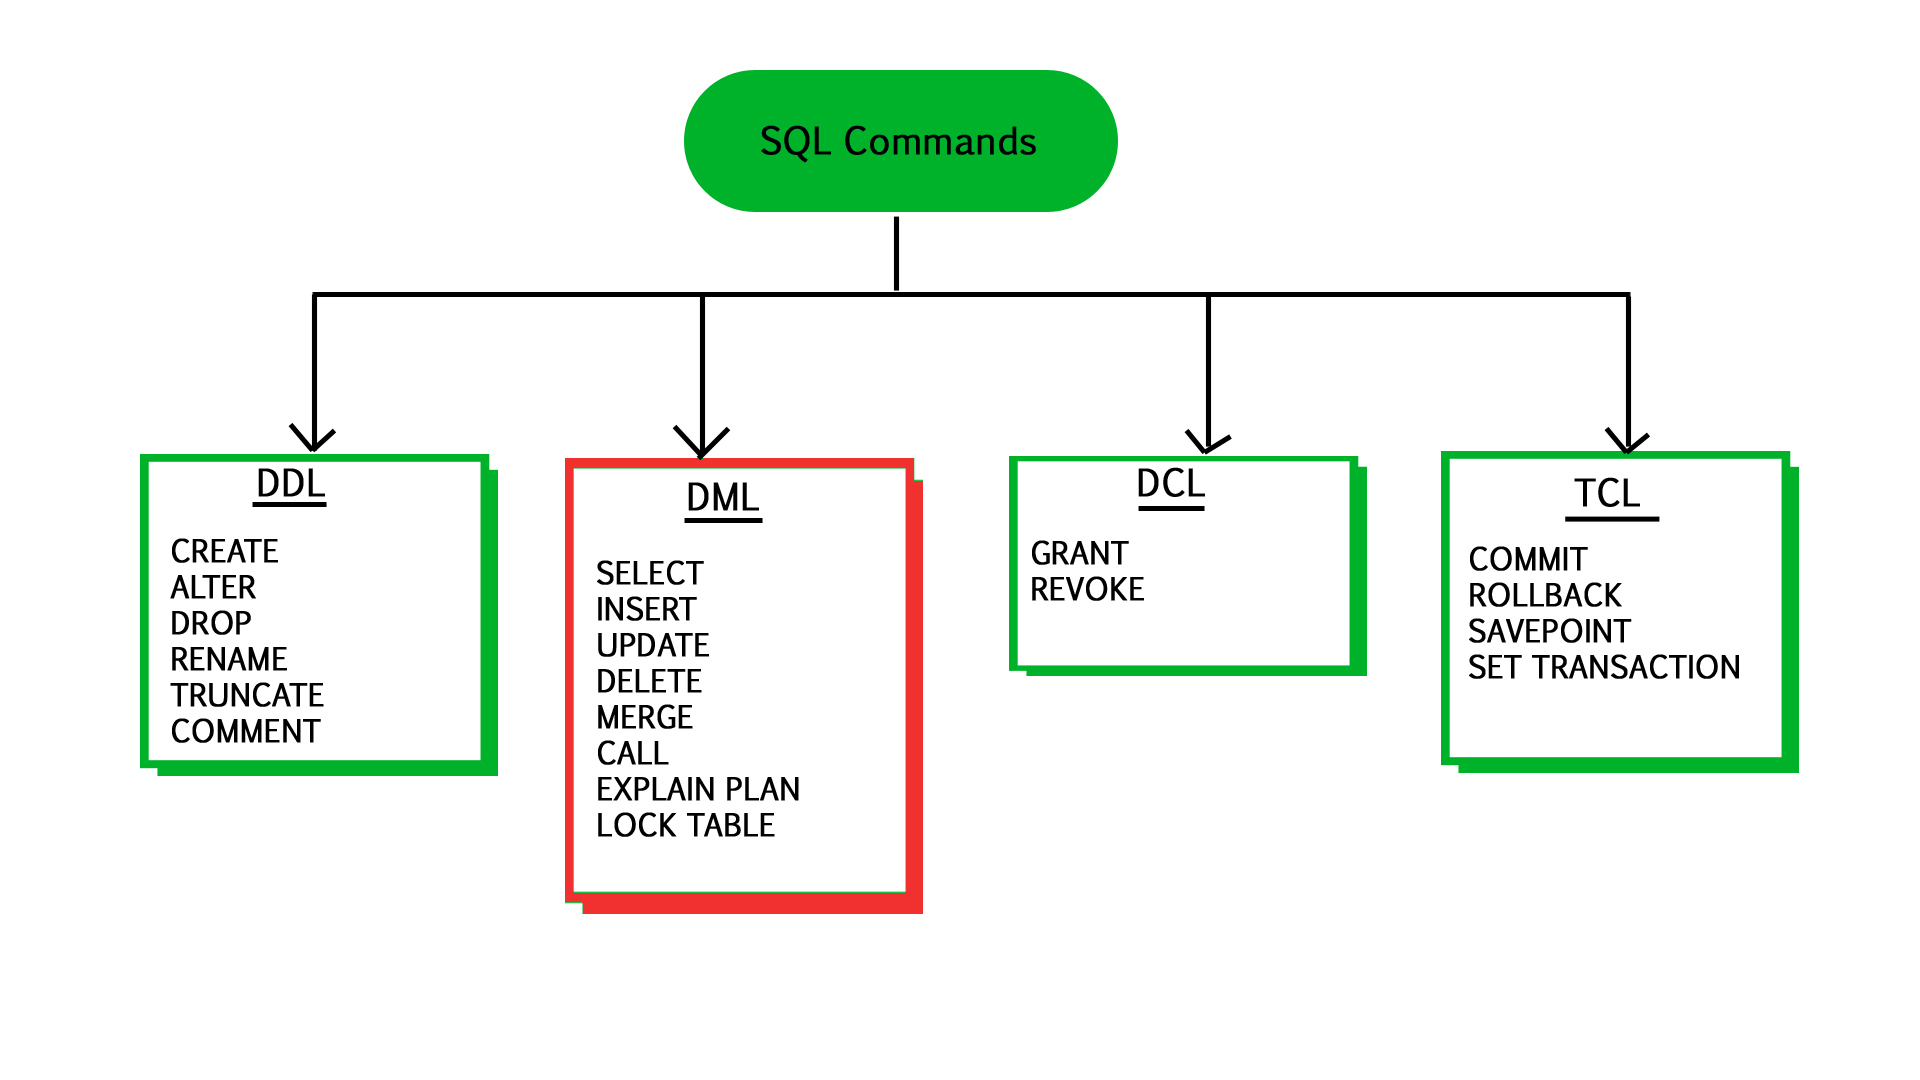
\includegraphics[width=0.75\textwidth]{img//sql-commands-dml.jpg}
  \label{img:dml}
\end{figure}

% ############################### FOR UPDATE ###############################
\subsection{FOR UPDATE}
\label{sec:dml.for_update}
\inputsql{code/dml/for_update.sql}

% ################################ INTERVAL ################################
\subsection{INTERVAL}
\label{sec:dml.interval}
\inputsql{code/dml/interval.sql}

% ################################ TO_CHAR ################################
\subsection{TO\_CHAR}
\label{sec:dml.to_char}
\inputsql{code/dml/to_char.sql}